%!TEX root = thesis.tex
\label{ch:prototype3}
The third approach to creating AHIs that we presented in chapter~\ref{ch:adhoc} was to construct the interface on the spot.
Of the three approaches this is the one that we have explored the least.

We presented this approach as the vision of interfaces that could be created from whatever you have at hand and creating the needed interface on the spot, pointing to a very palpable and literal version of ad hoc.
In this scenario it is solely up the user as to how the interface should behave, look and feel and while the interface should be easy to construct, it should be just as easy to deconstruct after it is no longer needed.

While the idea is intriguing, how do you go about making such a system?

\section{Related work}
We have done a few, though a bit cursory, experiments to explore the concept.
The main challenge has been to find materials, or a generic enough platform, that allows you to create objects or environments with interactive capabilities from \emph{whatever is immediately available}. 

There exist various physical ``frameworks'' or assembly kits that incorporates at least some of the aspects that we see in this approach to creating AHIs, in the sense that they provide building blocks or a general platform for creating interactive interfaces, that can be dismantled after use.

Examples of the assembly kit approach can be seen in Topobo \citep{raffle2004topobo}, seen in figure~\ref{topobo}, and Block Jam \citep{newton2003block}, seen in figure~\ref{blockjam}, where the focus is on the topological assembly of the different components of the system. 
Topobo is a physical 3D modelling system where the individual components have kinetic memory. 
The setup employs a mix of passive and active elements where the active components can record kinetic movement and play it back.
The kinetic outcome will then be based on how the different active and passive components are assembled.

Block Jam is a system that uses an array of physical blocks to create a dynamic and tangible sequencer.
In Block Jam the specific positioning of the individual blocks varies the auditive outcome, so while the blocks in themselves does nothing, the collection of blocks forms up an ad hoc dynamic sequencer.
Common for these two examples is that the individual components in the systems, while being part of a larger collection, are non customizable stand-alone object and that it is the topology of the assembly that defines the interactive capabilities.

\begin{figure}[h]
\centering
\begin{minipage}[t]{.44\textwidth}
  \centering
  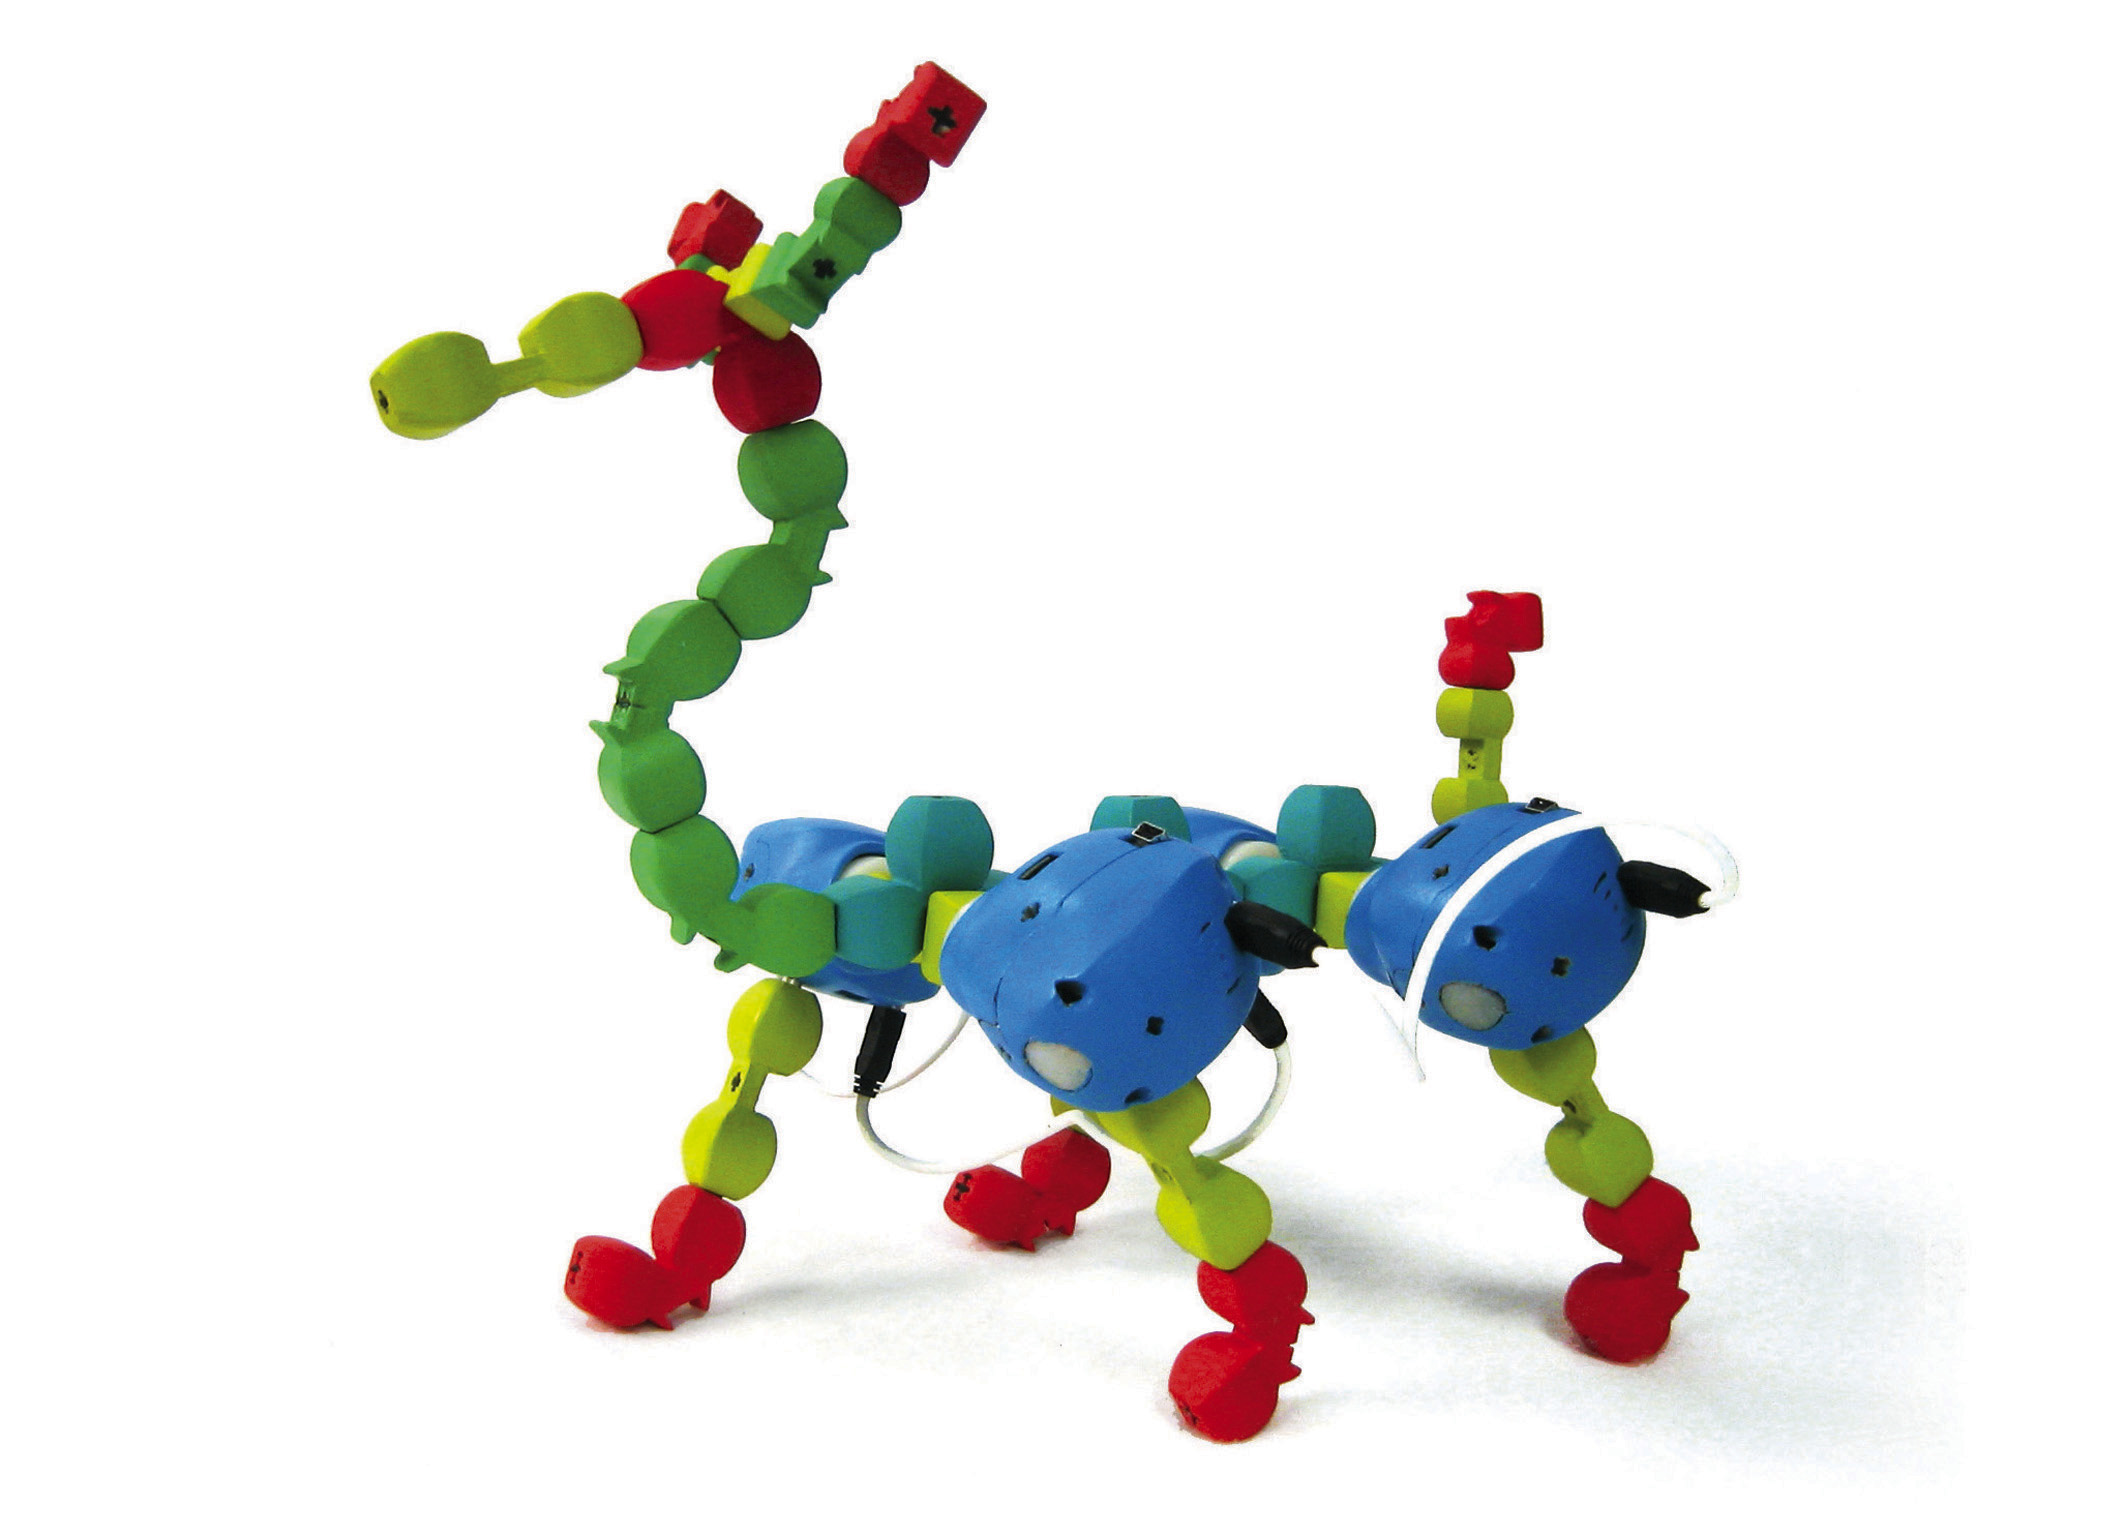
\includegraphics[width=\linewidth]{figures/proto3/topobo}
  \caption{Topobo, a kinetic 3D modelling system \citep{raffle2004topobo}.}
  \label{topobo}
\end{minipage}%
\hspace{0.02\textwidth}
\begin{minipage}[t]{.44\textwidth}
  \centering
  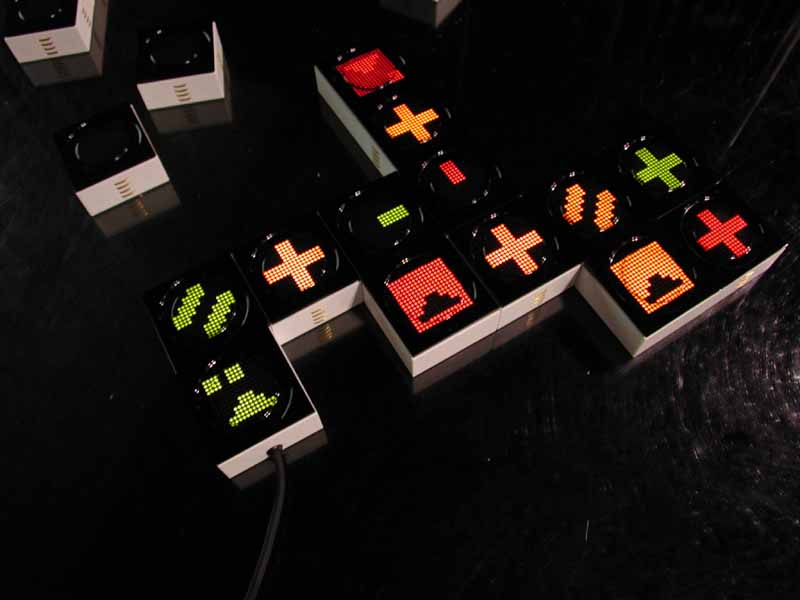
\includegraphics[width=\linewidth]{figures/proto3/blockjam}
  \caption{Block Jam, a dynamic tangible sequencer \citep{newton2003block}.}
  \label{blockjam}
\end{minipage}
\end{figure}

A more general purpose approach is seen in physical computing platforms such as Arduino, which is a prototyping platform for electronics and one we have used a lot in our prototype work for this thesis, and LEGO Mindstorms\footnote{http://mindstorms.lego.com/en-us/default.aspx} which is a programmable robotics platform.
Compared to Topobo and Block Jam, much less details are abstracted away on the two platforms and therefore gives an increased focus on digital programmability and on more generic components.
As such a specific component does not have a specific application purpose in mind and the topological placement of components are not defined by the platform -- of course wires, actuators, sensors, gears, wheels, and so on, have to be assembled correctly to function.
\blank
On a even more basic level we see different materials that have interesting qualities in relation to AHIs on their own.
This could be materials such as smart memory alloys or conductive paints, that, while they need for advanced functionality need a supporting infrastructure, have interesting capabilities in them selves with just the addition of electricity.

Here we will highlight one such material which is a conductive paint made by Bare Conductive\footnote{http://www.bareconductive.com}.

We see two overall basic options for using a paint like this.
Firstly as a connector where the paint either acts as a wire between two points or as a switch.
Secondly the paint can work as a variable resistor as the paint itself is resistive inversely proportional to the cross sectional area\footnote{http://www.bareconductive.com/file/2013-technicaldatasheet-bareconductivepaint-pdf}. 
This means that a thin line will have a higher resistance than a wide line of the same length.

Although this is some quite simple mechanics there are examples of clever uses of these two properties.

\begin{figure}[h]
  \centering
  \begin{minipage}[b]{.8\textwidth}
    \centering
    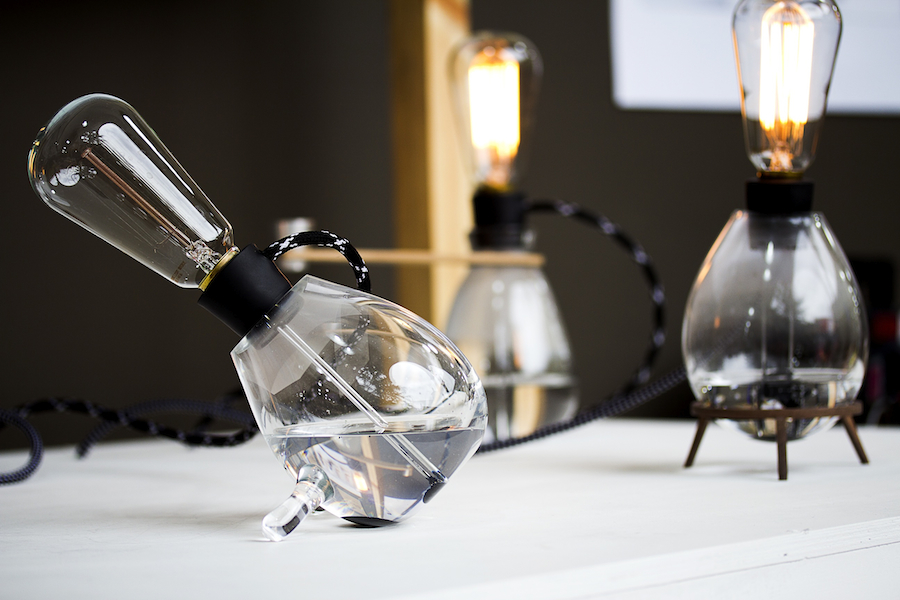
\includegraphics[width=.7\linewidth]{figures/proto3/liquidity_lamp}
	\caption{The Liquidity Lamp, an alternative use of conductive paint}
   \label{liquidity_lamp}
   \end{minipage}
\end{figure}

A collaboration between the creators of Bare Conductive and musician Calvin Harris resulted in the Humanthesizer, a human synthesizer where people painted in conductive ink formed the instruments for a performance\footnote{http://cargocollective.com/foamagency/Calvin-Harris-Humanthesizer}.
So here the paint is used as a wire, but between people instead of objects.

Another example is The Liquidity Lamps \footnote{http://pstevensonkeating.co.uk/portfolio/liquidity} by Patrick Stevenson-Keating, seen in figure~\ref{liquidity_lamp}, where the paint is used in combination with transparent oil to create a liquid switch that, by tilting it, turns the lamp on and off.

The conductive capabilities can also be used to create painted capacitors\footnote{http://www.bareconductive.com/painting-a-capacitor} where it is shown that a paper painted on both sides can be used as a capacitor, as the paper will act as an insulator between the two conductive sides and store a small amount of energy.
Also inherent resistance in the paint also allow for painted potentiometers as a simple painted line will have increasing resistance and thereby act as a variable resistor along the line.

Here we have shown three different categories of physical frameworks or assembly kits that can potentially be used to construct applications with ad hoc capabilities, from the very specific in Topobo and Block Jam, to the general in Arduino and Mindstorms, and least the very elementary in Bare Conductive.

In the next section we will present a cursory exploration of the possibilities of using a paint like Bare Conductive in the domestic setting to create AHIs.

\section{Exploration}
We have explored the use of Bare Conductive, an electric water-based paint, as a material for creating AHIs on the spot.
This electrical paint has some interesting properties as it is easily applied and dries quickly but at the same time, because it is water-based, can be removed with a wet cloth.
This fits well with our idea of an interface that is quick to make and quick to erase.

Inspired by Brand's earlier mentioned six S's \citep{brand1995buildings} we have envisioned a concept where we, instead of hiding it, try to expose the infrastructures of the house.
It is the norm to hide as much of the ``working guts'' of a building from sight.
Electrical wiring and plumbing are embedded into the building itself hindering easy change or modification to these systems.
Our idea is to bring down these services to the layer of Stuff where continuous changes and adaptations can be made as needed.
At the same time it is a move against the tendency of always hiding away the complexity of things behind polished surfaces, instead showing off the complexity as an aesthetic intellectual quality, combining the raw functionality of the service with the expressiveness of paints.

We have taken an offset in the wiring of the house and envision a concept where the wires and switches in the house can be painted on the walls with both the traditional functionality of wires, but also the added ability to create visual interactive expressions.
As the shape of the paint will affect the resistance, as mentioned earlier, this will provide the ability to, at least in some fashion, have the visual expression correlate with the interactive capabilities, combining aesthetic expression with functionality.

We have made a simple video prototype showing the possibility of creating a dynamic light switch on the wall and removing it again.
In figure \todo{ref} a room is shown with its wiring exposed to the inhabitants as a mix of functionality and wall art that can be remade or adapted as they see fit.

So can a paint like Bare Conductive provide ad hoc capabilities?

\section{Discussion}
When we started out our exploration of paint as a medium for AHIs we thought that it would be easy to conceptualize and show off some compelling and interesting examples of how this could be used.
We wanted to focus less on the supporting infrastructure and more on the possibilities of using paint, more or less exclusively, as the interface and as the defining property for how the interaction worked. 
However we quickly became severely limited by the fact that our material only supports conduction and resistance and therefore many of the usually given components in physical computing, such as transistors, gates, diodes etc., is not possible to make on the spot, without supporting infrastructure.  

\todo{interesting stuff goes here}

We still \todo{stuff here needs fixing} that the idea of creating the actual material interface on the spot, where the interface is fashioned to your current needs and shaped to your liking by yourself, is wildly enticing, though it might not be entirely realistic.
There is a beauty in the idea of an interface constructed from a simple material, that can be washed away when it is no longer needed, but still provide interesting interacting capabilities.
In the end though you will always be constrained by the underlying system as there will always be a need for infrastructure to realise real life versions of concepts such as the ones we have presented here.

\begin{verbatim}
physical programming - digital programming
related work : topobo, surflex, music blocks
bare paint exploration
the need for infrastructure - will always be limited by the underlying system
leading to AHIs
Inspired by the domain, bring the infrastructure out from the walls,
 aesthetics and functionality
 deconstruct
\end{verbatim}